\chapter{Model Diagnostics \& Further Identified Objects}

\section{Further Model Diagnostics}\label{further-diagnostics}
\noindent In Section \ref{diagnostics} we present diagnostic properties of our model. These include the accuracy measurements, purity measurements as well as confusion matrices at different cutoffs of our model. Here, we present the Receiver Operating Characteristic (ROC) curves, the precision-recall (PR) curves, and measures of true and false positive rates vs the cutoff threshold.

Figure \ref{fig:pr-roc-curves} shows the ROC and PR curves of the final \texttt{Zoobot} model we applied to the the \emph{Hubble} archives. The ROC shows the rate of change of finding true positives and false positives with changing cutoff. The PR curve shows the changes of precision against recall. Precision is the ratio of true positives (interacting galaxies correctly predicted as so) to the sum of true and false positives (non-interacting galaxies incorrectly predicted as interacting). The recall is then the ratio of true positives to the sum of true positives and false negatives (interacting galaxies that have been misclassified as non-interacting). The red crosses in both plots shows how the model was behaving when we use a cutoff of 0.95. 

These are both as expected. Both curves show that the model behaves well, and are much better than a random classifier (which would have a 1:1 relation). The ROC plot shows that we are minimising our false positive rate when using a prediction score cutoff of 0.95. However, we are misclassifying approximately 50\% of interacting galaxies as non-interacting galaxies. The contamination rate in our final catalogue (False Positives rate) will be very low (close to zero in this ideal validation set). The PR curve shows a similar result. Here, we are operating with a high precision (finding a pure catalogue) while keeping our recall minimal. 

We also present the changing F1 score for the model used in this work, shown in Figure \ref{fig:f1-score}. The F1 score is twice the ratio of precision multiplied by recall upon precision summed to recall. This combines our measure of accuracy and purity into a single metric. The cutoff we use in this work is at the point where the F1 score has began to decline. This is because we are beginning to lose recall rapidly, but gaining significantly in precision. As discussed in Section \ref{diagnostics}, this was an acceptable trade off in this work for a very large, pure interacting galaxy catalogue.

\begin{figure*}
  \centering
  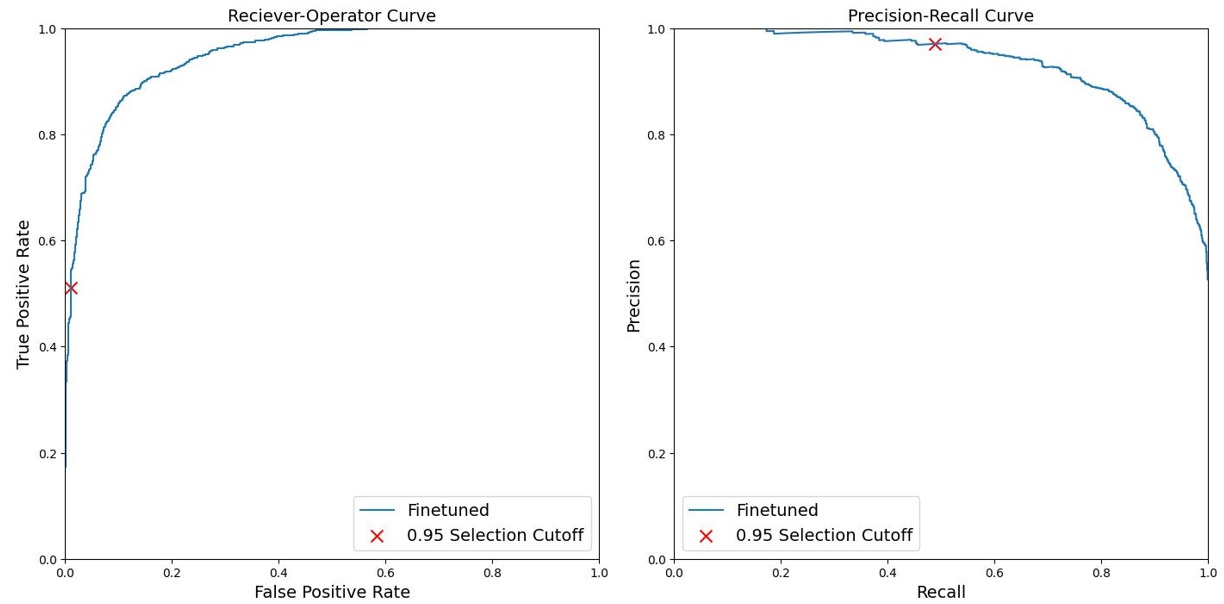
\includegraphics[width = 0.95\textwidth]{Chapter2/figures/fig14.jpg}
  \caption{The Receiver-Operator and Precision-Recall Curve for the \texttt{Zoobot} model that was used to explore the Hubble archives. The blue curves are the measured curves. These curves measure the relevant rates or characteristics based on the changing cutoff applied to how \texttt{Zoobot} defines an interacting galaxy. The red crosses are where the prediction score cutoff is for this work. We can see in the Reciever-Operator Curve that the prediction score cutoff we use would have an incredibly low false positive rate, while it would be misclassifying $\approx$50\% of interacting galaxies. This also shown in the precision recall curve where our recall is $\approx$50\%.}
  \label{fig:pr-roc-curves}
\end{figure*}

\begin{figure*}
    \centering
    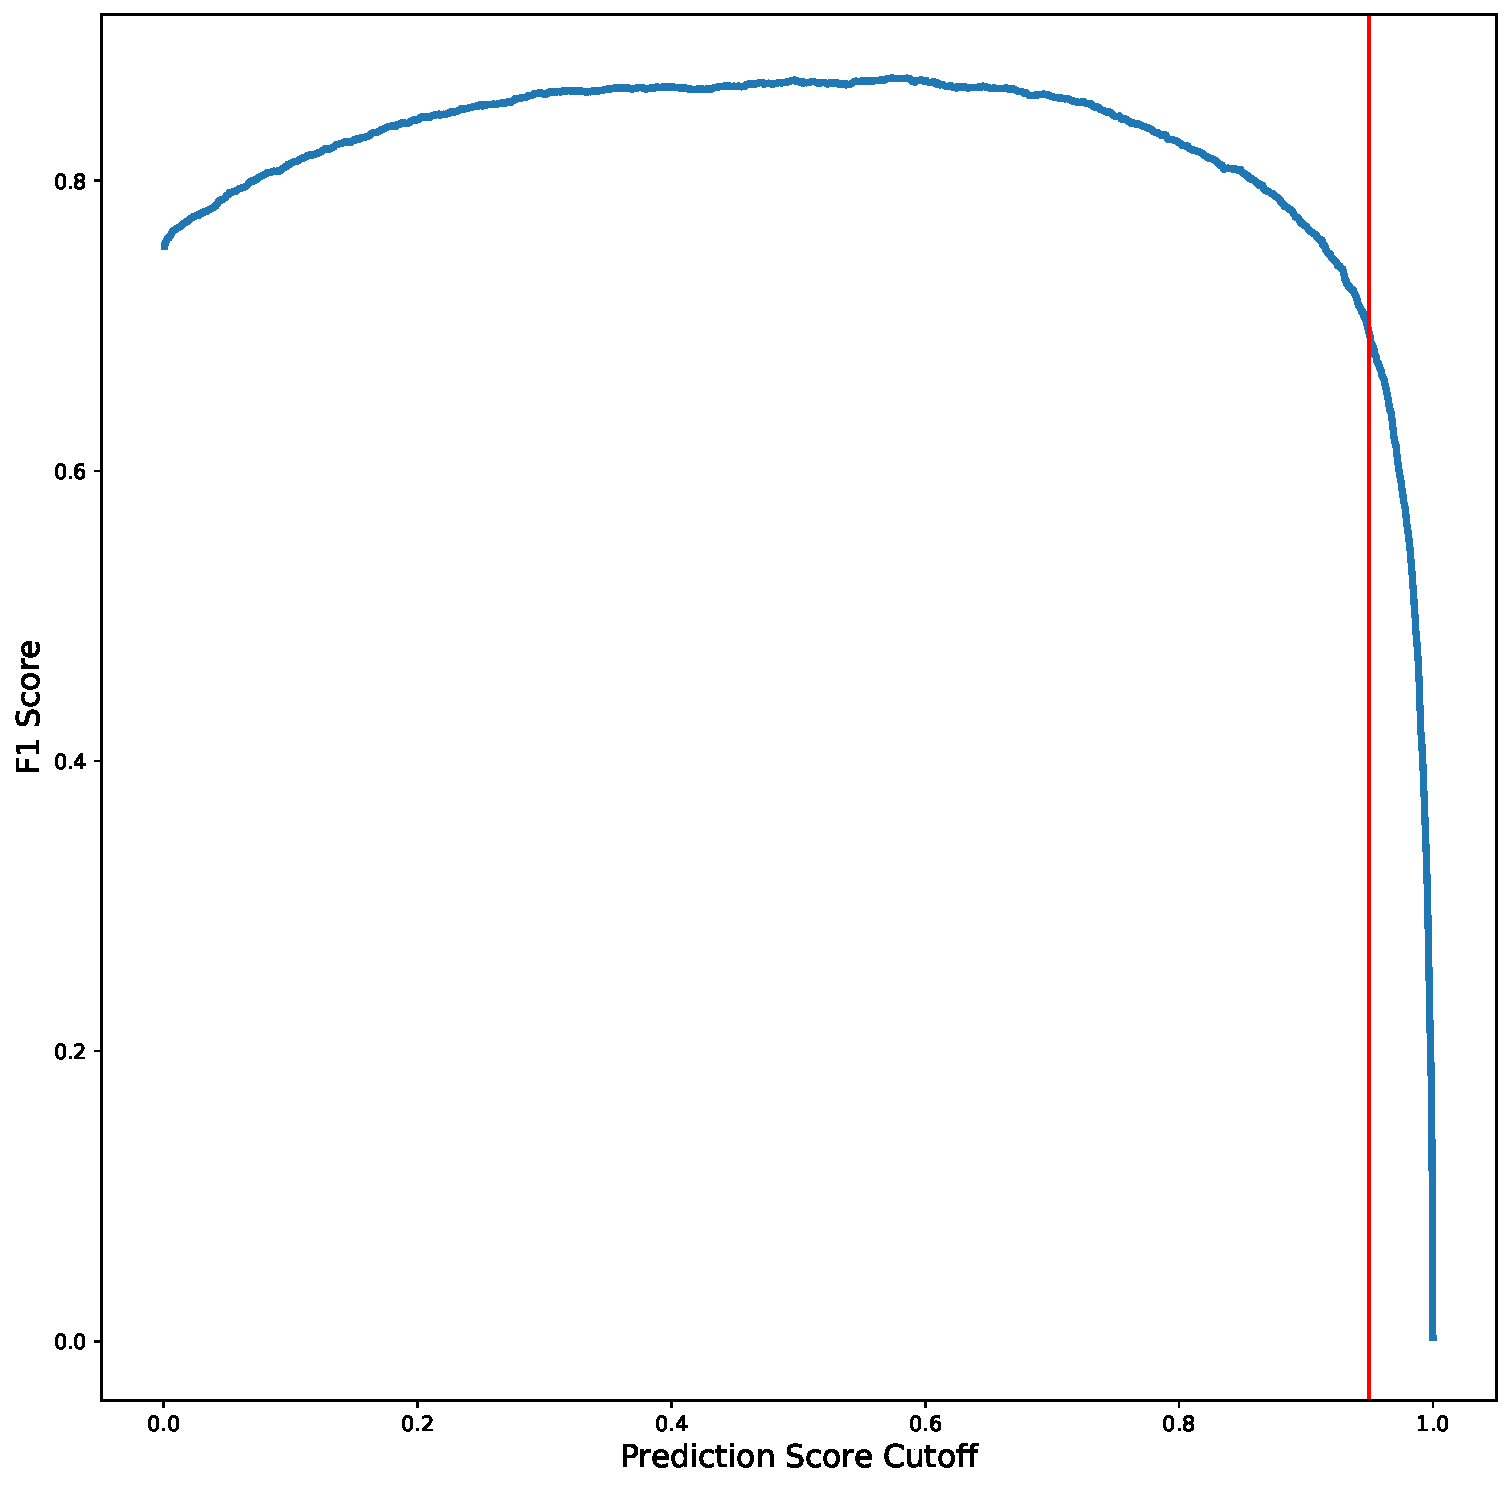
\includegraphics[width = 0.65\textwidth]{Chapter2/figures/fig15.pdf}
    \caption{The F1 score found during the diagnostics of the model used in this work. The F1 score is a measure combing the measure of accuracy and purity into one metric. The cutoff we use is at the point where the F1 score begins to rapidly decline. This point is shown by the red vertical line.}
    \label{fig:f1-score}
\end{figure*}

\section{Examples of Sources with 3-Band Information}\label{colour-images}
\noindent Of the full catalogue of 21,926 interacting systems, only 1336 of them had got all 3-band information. Six examples are shown in Figure \ref{fig:colour-images}. These were created using the \citet{lupton_04} algorithm, with a scaling factor $Q = 2$ and $\alpha = 0.75$, with ($F814W$, $F606W$, $F475W$) as RGB channels and multiplicative factors of (1.25, 0.95, 2).

\begin{figure*}
  \centering
  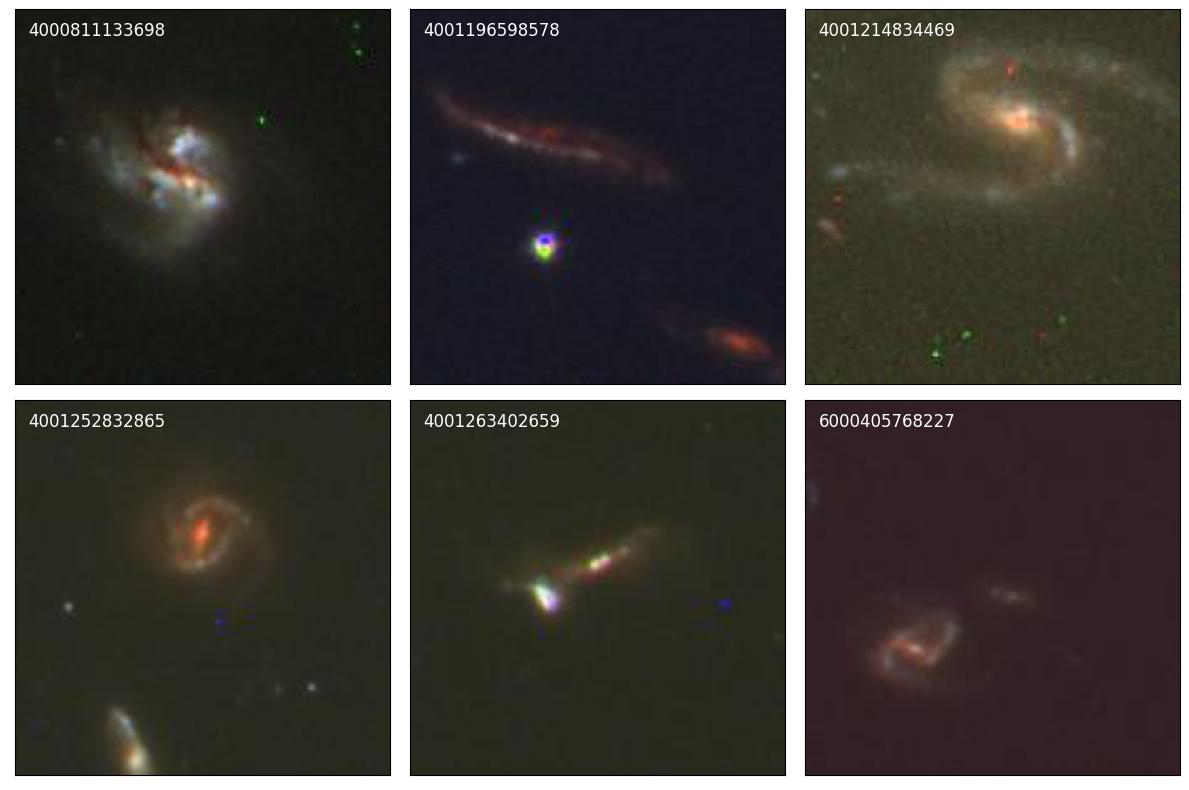
\includegraphics[width = 0.85\textwidth]{Chapter2/figures/fig16.jpeg}
  \caption{Example of six interacting systems in the catalogue with full 3-band imagery.}
  \label{fig:colour-images}
\end{figure*}

\section{Unknown Objects}\label{unknown-object}
\noindent From the final catalogue, there were six sources which we could not visually identify. These objects were also not referenced anywhere in the astrophysical literature. $F814W$ cutouts of the six objects are shown in Figure \ref{fig:unknown-images}. Their Source IDs are shown in the upper left of each image, and a separate catalogue has been released of these with all other objects. This catalogue can be found at the data release on Zenodo.

Four of the six objects (40001156424176, 4001368788120, 4001418076626 and 6000398415347) have a bright central source, followed by a low-surface brightness tail. Initially, it was assumed that these were solar system objects such as comets. This, however, could not be confirmed. The first of these four sources is also thought to potentially be a highly disruped system with a significantly elongated tidal feature. The final two unknown sources (6000186797547 and 6000341449179) have no clear central source, though there is extended structure to them. These are likely to be highly irregular galaxies, but no confirmation could be found.

These objects are released to the community for identification and investigation, as the authors cannot find definitive agreement on what they are. 

\begin{figure*}
  \centering
  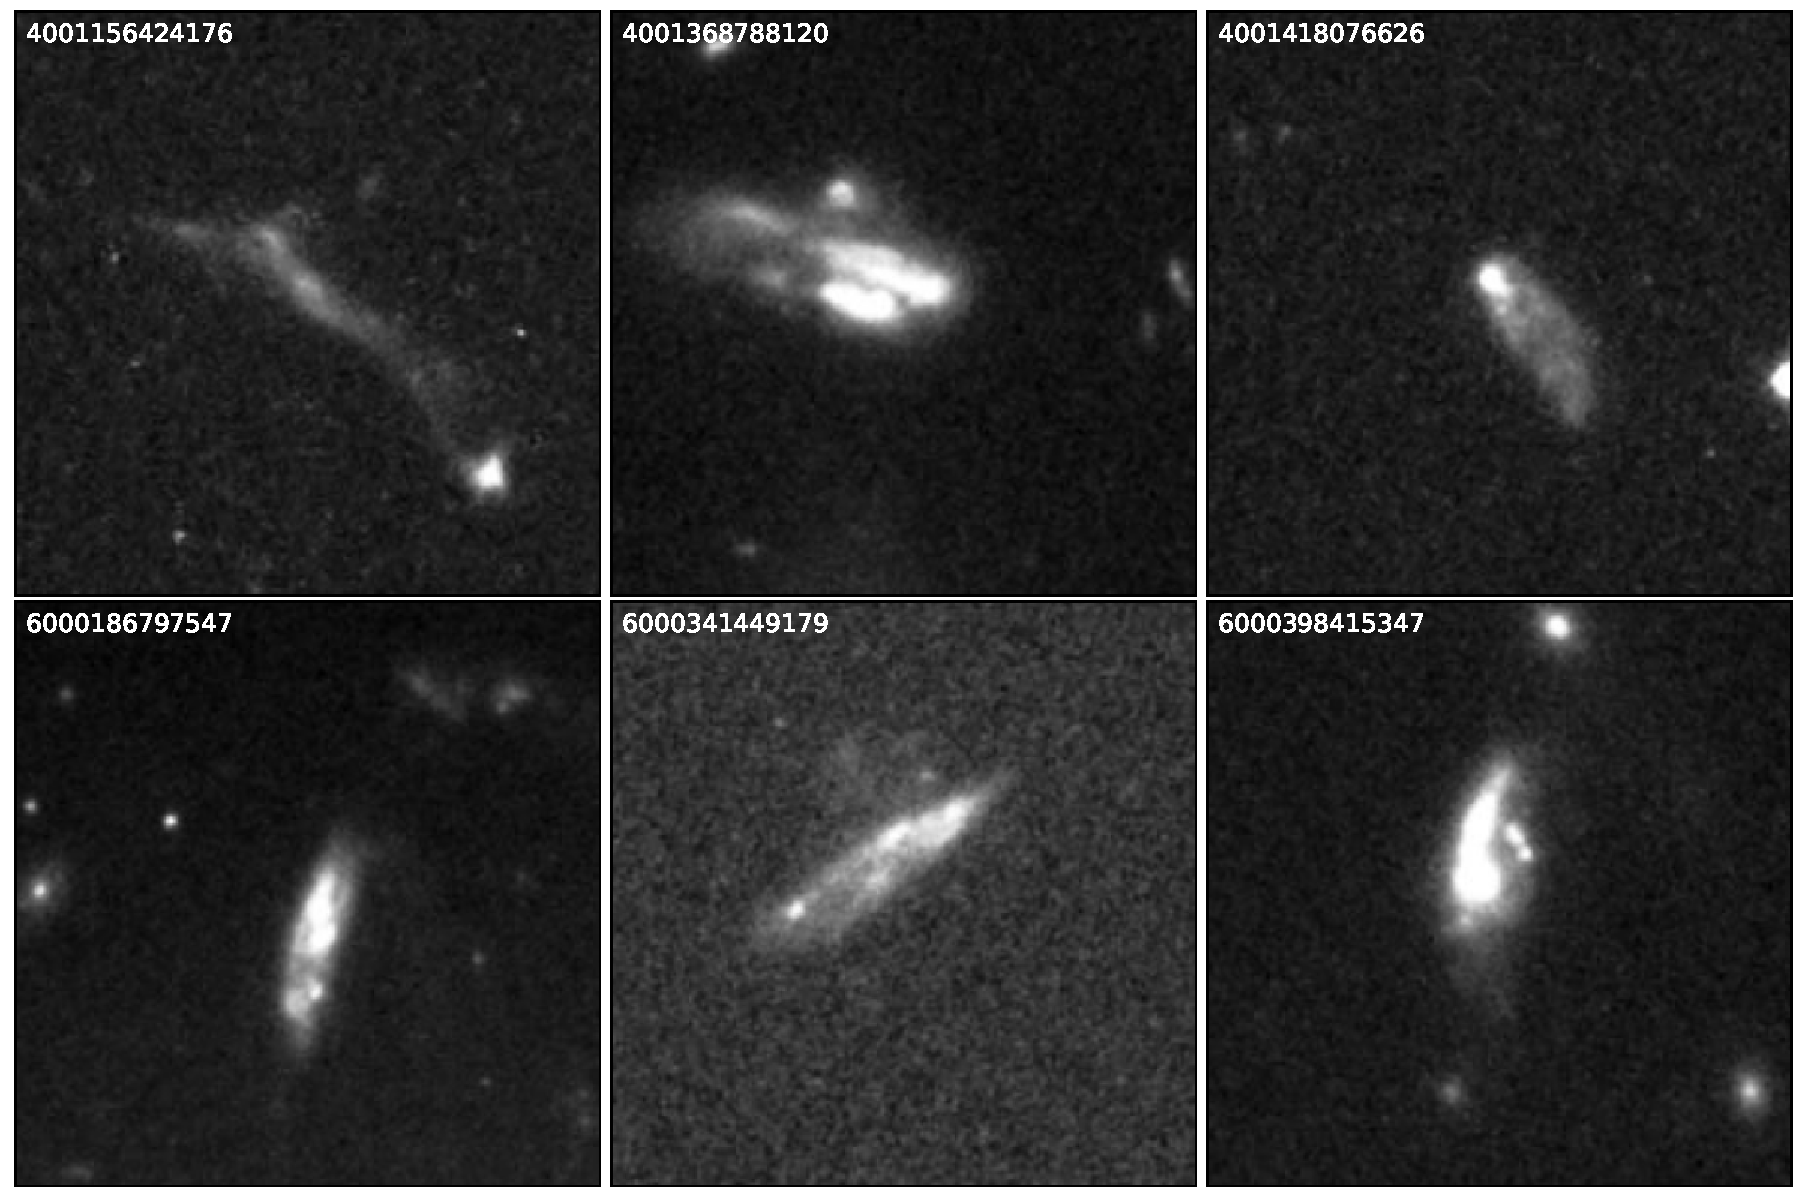
\includegraphics[width = 0.85\textwidth]{Chapter2/figures/fig17.pdf}
  \caption{The six unknown systems found in this work. These have no reference in Simbad or in NED, and their morphology could not be classified by the authors. Investigation into these six objects are presented to the community, with the authors hoping that future work and investigation of them can be conducted by them.}
  \label{fig:unknown-images}
\end{figure*}

\section{Acknowledging PIs}
\noindent In the final section of this work, we wish to acknowledge all of the PIs whose observations we have used. A machine readable table containing the proposal IDs, the DOIs and the references (if provided/found) is presented with this work. Table \ref{tab:pis} shows the first twenty observations used in this work and is an example of this table.

\begin{table}
\centering
	\begin{tabular}{ccccc}
	Proposal ID & Observation ID & Observation Date & DOI & references \\
	    8183       &   hst\_8183\_54\_acs\_wfc\_f814w\_j59l54 &       18/07/2002 &    https://doi.org/10.5270/esa-88k8vcj & \\
	    9075       &   hst\_9075\_2a\_acs\_wfc\_f814w\_j6fl2a &       24/07/2002 &    https://doi.org/10.5270/esa-gsxhb4b & \\
	    9351       &   hst\_9351\_11\_acs\_wfc\_f814w\_j8d211 &       31/03/2003 &    https://doi.org/10.5270/esa-5lba8bo & \\
	    9361       &   hst\_9361\_03\_acs\_wfc\_f814w\_j8d503 &       22/07/2003 &    https://doi.org/10.5270/esa-ecmnqgh & \\
	    9363       &   hst\_9363\_09\_acs\_wfc\_f814w\_j8d809 &       02/07/2002 &    https://doi.org/10.5270/esa-ethtec5 & \\
	    9367       &   hst\_9367\_02\_acs\_wfc\_f814w\_j8ds02 &       10/06/2003 &    https://doi.org/10.5270/esa-3j404ll & \\
	    9373       &   hst\_9373\_02\_acs\_wfc\_f814w\_j6la02 &       05/07/2002 &    https://doi.org/10.5270/esa-ztsq94u & \citet{Rejkuba_05}\\
	    9376       &   hst\_9376\_02\_acs\_wfc\_f814w\_j8e302 &       13/07/2002 &    https://doi.org/10.5270/esa-h90iavd & \citet{Keel06}\\
	    9381       &   hst\_9381\_02\_acs\_wfc\_f814w\_j8fu02 &       13/03/2003 &    https://doi.org/10.5270/esa-vlapyea & \\
	    9400       &   hst\_9400\_04\_acs\_wfc\_f814w\_j6kx04 &       29/05/2003 &    https://doi.org/10.5270/esa-39rnout & \\
	    9403       &   hst\_9403\_02\_acs\_wfc\_f814w\_j8fp02 &       09/07/2002 &    https://doi.org/10.5270/esa-k5mv9ct & \\
	    9405       &   hst\_9405\_6k\_acs\_wfc\_f814w\_j8iy6k &       22/05/2003 &    https://doi.org/10.5270/esa-zy9phm1 & \\
	    9409       &   hst\_9409\_03\_acs\_wfc\_f814w\_j6n203 &       29/06/2003 &    https://doi.org/10.5270/esa-vjngw7r & \citet{goudfrooij04}\\
	    9411       &   hst\_9411\_09\_acs\_wfc\_f814w\_j8dl09 &       11/02/2003 &    https://doi.org/10.5270/esa-debpiln &  \\
	    9427       &   hst\_9427\_13\_acs\_wfc\_f814w\_j6m613 &       21/10/2002 &    https://doi.org/10.5270/esa-bw1b97v &  \\
	    9438       &   hst\_9438\_01\_acs\_wfc\_f814w\_j6me01 &       16/01/2003 &    https://doi.org/10.5270/esa-e5eaam5 & \citet{gregg17}\\
	    9450       &   hst\_9450\_02\_acs\_wfc\_f814w\_j8d402 &       25/08/2002 &    https://doi.org/10.5270/esa-9ttmykz & \citet{york05}\\
	    9453       &   hst\_9453\_02\_acs\_wfc\_f814w\_j8f802 &       03/12/2002 &    https://doi.org/10.5270/esa-1xvyjfy & \citet{brown03}\\
	    9454       &   hst\_9454\_11\_acs\_wfc\_f814w\_j8ff11 &       23/03/2003 &    https://doi.org/10.5270/esa-xsdowj9 &  \\
	\end{tabular}
\caption{Twenty example of the accompanying data table of observations used.} 
\label{tab:pis}
\end{table}